\documentclass[
	classe=$1^{ere}$STI2D
]{coursclass}

\usepackage{annotate-equations}

\newcommand{\makegrid}[2]{
	\foreach \y in {-#1, ..., #1} {
		\draw[ultra thin] (-#2,\y) -- (#2,\y);
		\ifthenelse{\equal{\y}{0}}{}{
		\draw[thick] (-0.2,\y) node[left] {\y} -- (0,\y);
		}
	}
	\foreach \x in {-#2, ..., #2} {
		\draw[ultra thin] (\x,-#1) -- (\x,#1);
		\ifthenelse{\equal{\x}{0}}{}{
		\draw[thick] (\x,-0.2) node[below] {\x} -- (\x,0);
		}
	}
	\node[below,left] at (-0.2,-0.3) {$0$};
	\draw[very thick,\myArrow] (-#2 - 0.3,0) -- (#2 + 0.5,0);
	\draw[very thick,\myArrow] (0,-#1 - 0.3) -- (0,#1 + 0.5);
}

\title{Cours Chapitre 2}
\author{Généralités sur les fonctions}
\date{}

\begin{document}

\maketitle

\begin{definition}[Fonction]
	Une \textbf{fonction} numérique est un procédé qui à tout nombre associe un \textit{unique} autre nombre.

	La fonction est généralement notée $f$, le nombre de départ est noté $x$ et le nombre obtenu est noté $f(x)$. On le lit « $f$ de $x$ », ou encore « $f$ appliquée à $x$ ».

	On la note
	$$ f : x ↦ f(x) $$

	\begin{itemize}
		\item $f(x)$ est \textbf{l'image} de $x$ par la fonction $f$.

		      On représente une image par la lettre $y$, et on écrit alors \uline{$f(x) = y$}.
		\item $x$ est \textbf{\uline{un} antécédent} de $f(x)$ par la fonction $f$.
	\end{itemize}
\end{definition}

\begin{remarque}
	\begin{itemize}
		\item Pour un nombre donné $x$, il n'y a \uline{q'une seule image} $f(x)$.
		\item Pour un nombre donné $y$, il peut y avoir \uline{plusieurs antécédents} $x$ tels que $y = f(x)$.
	\end{itemize}
\end{remarque}

\begin{exemple}
	\begin{minipage}{0.7\linewidth}
		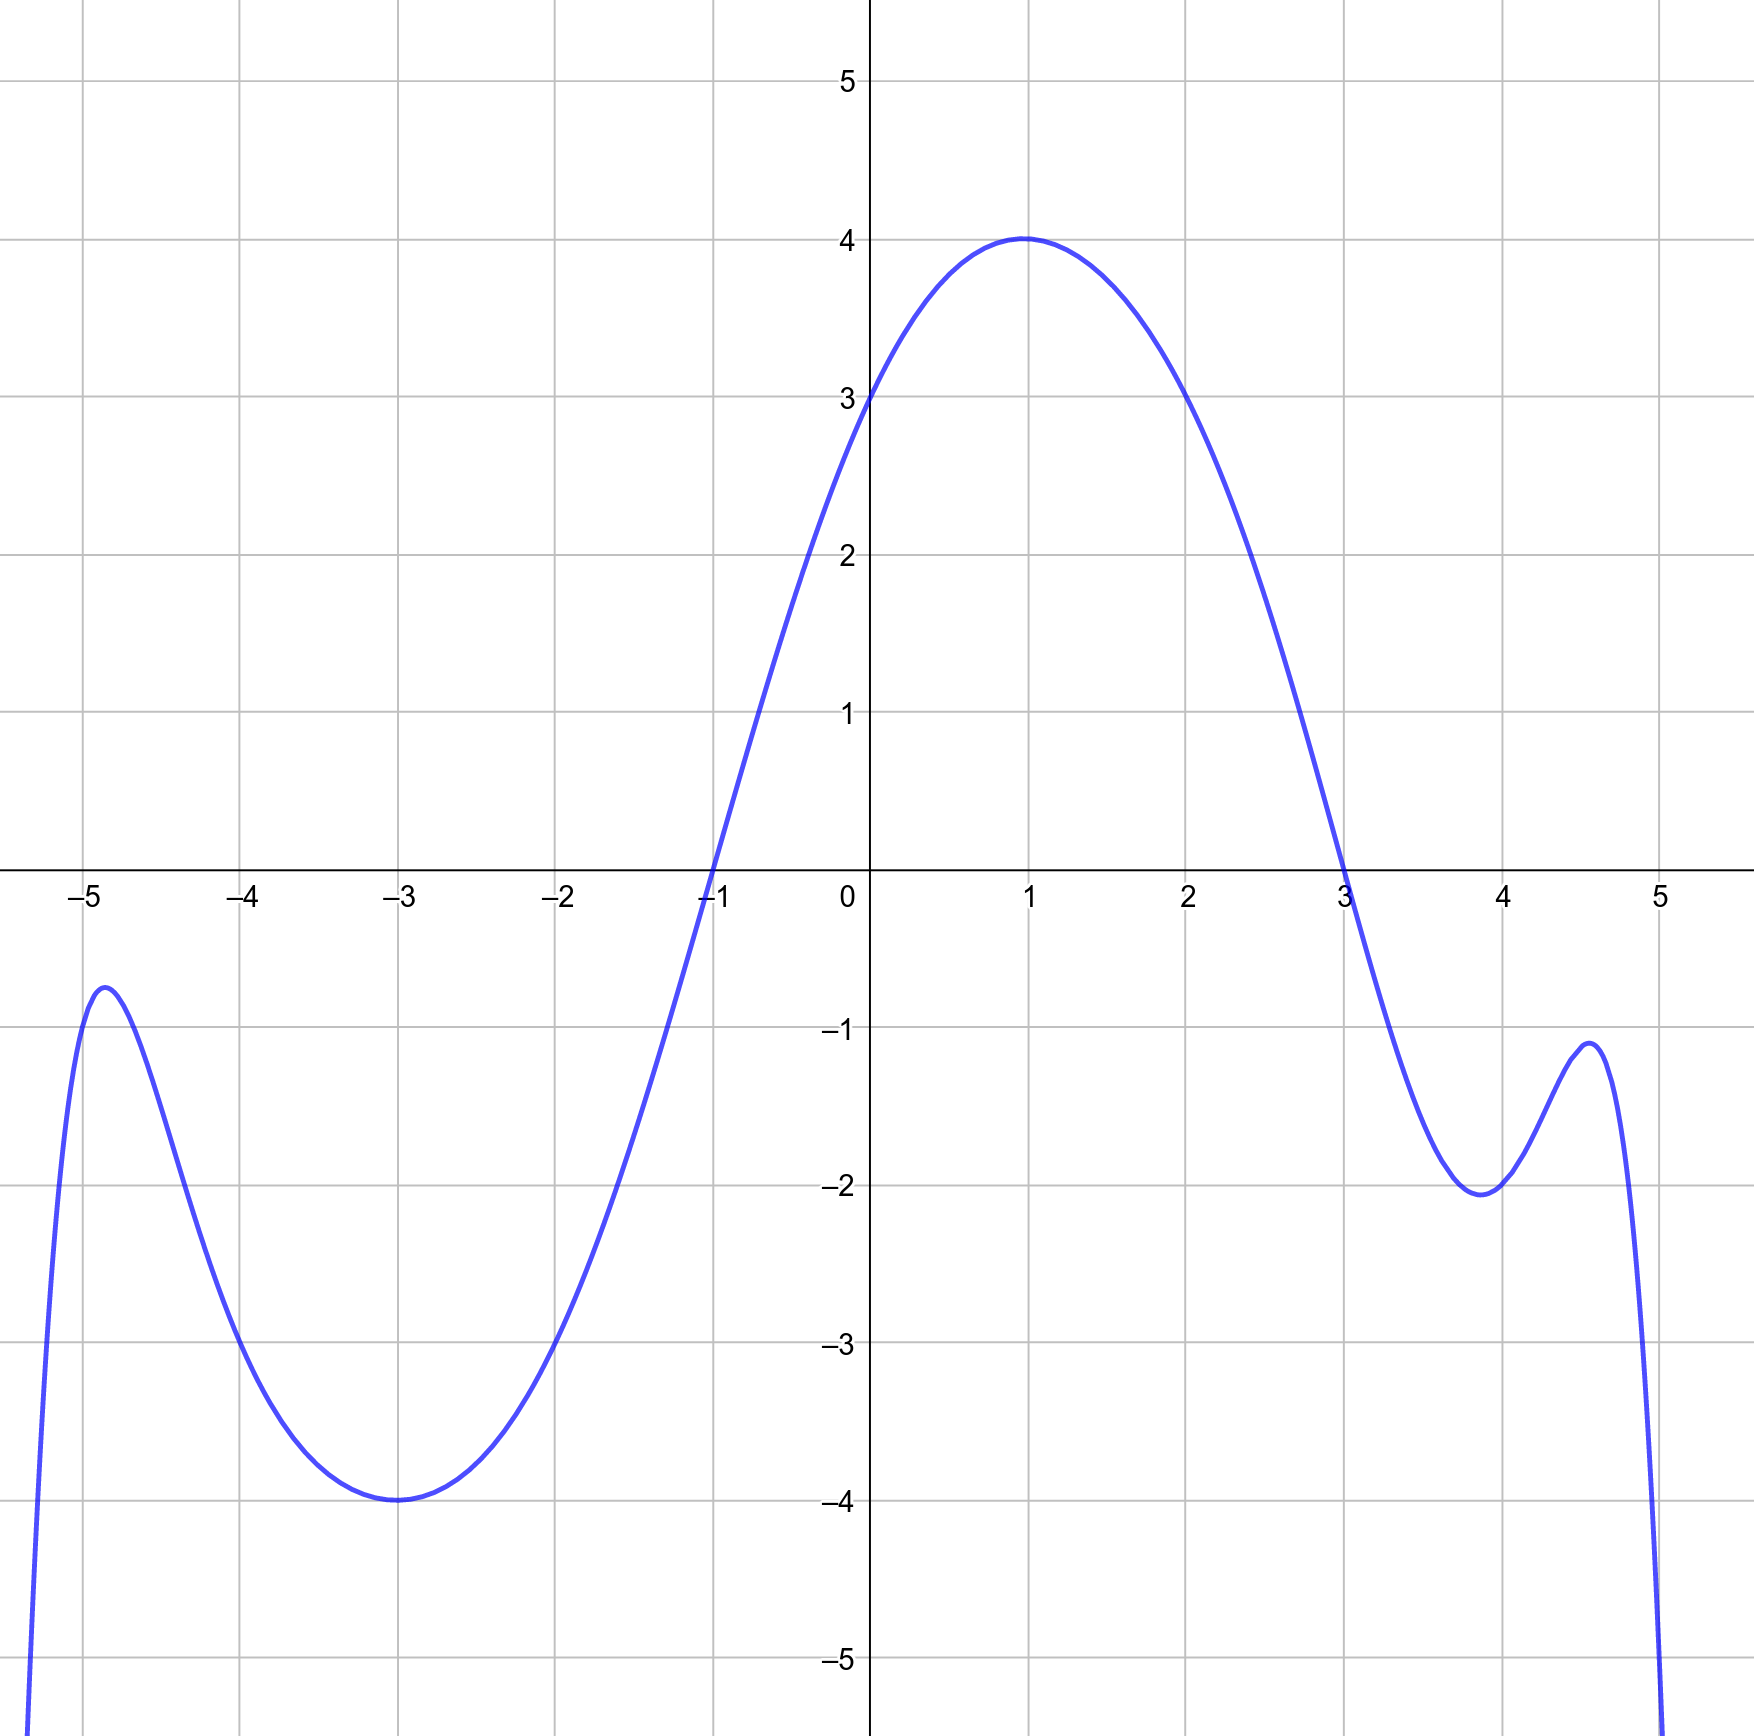
\includegraphics[width=\linewidth]{graphe 1.png}
	\end{minipage}
	\begin{minipage}{0.3\linewidth}
		\begin{center}
			\renewcommand{\arraystretch}{1.2}
			\begin{tabular}{|c|c|}
				\hline $x$  & $f(x)$ \\
				\hline $-5$ &        \\
				\hline $-4$ &        \\
				\hline $-3$ &        \\
				\hline $-2$ &        \\
				\hline $-1$ &        \\
				\hline $0$  &        \\
				\hline $1$  &        \\
				\hline $2$  &        \\
				\hline $3$  &        \\
				\hline $4$  &        \\
				\hline $5$  &        \\
				\hline
			\end{tabular}

			\begin{itemize}
				\item L'\textbf{image} de $2$ est .....\vspace{0.5em}
				\item L'\textbf{image} de $-1$ est .....\vspace{0.5em}
				\item Les \textbf{antécédents} de $4$ sont .........\vspace{0.5em}
				\item Les \textbf{antécédents} de $-3$ sont .........
			\end{itemize}
		\end{center}
	\end{minipage}
\end{exemple}

\end{document}